\section{Fractional QHE}

Experiments show that the filling factor $\nu$ takes not only integer values, but also fractions $\nu=\frac{1}{2}, \frac{2}{5}, ...$.
This can be partially explained by the creation of fractionally charged quasiparticles.
This effect is typically observed at very high magnetic fields.
Since none of the curves go beyond $\nu = 1$, a larger magnetic field would be required to observe fractional filling factors smaller than 1. In principle, fractional filling factors larger than 1 can also occur.
Fig. \ref{fig:FQHE} shows the Hall resistance for $1.4K$ and a gate voltage of $-0.25V$.
There are no plateaus visible at levels of a fractional $\nu$.
The resistances where a plateau should be visible for $\nu = 4/3$ and $\nu = 5/3$ are highlighted as an example.
\begin{figure}[h]
    \centering
    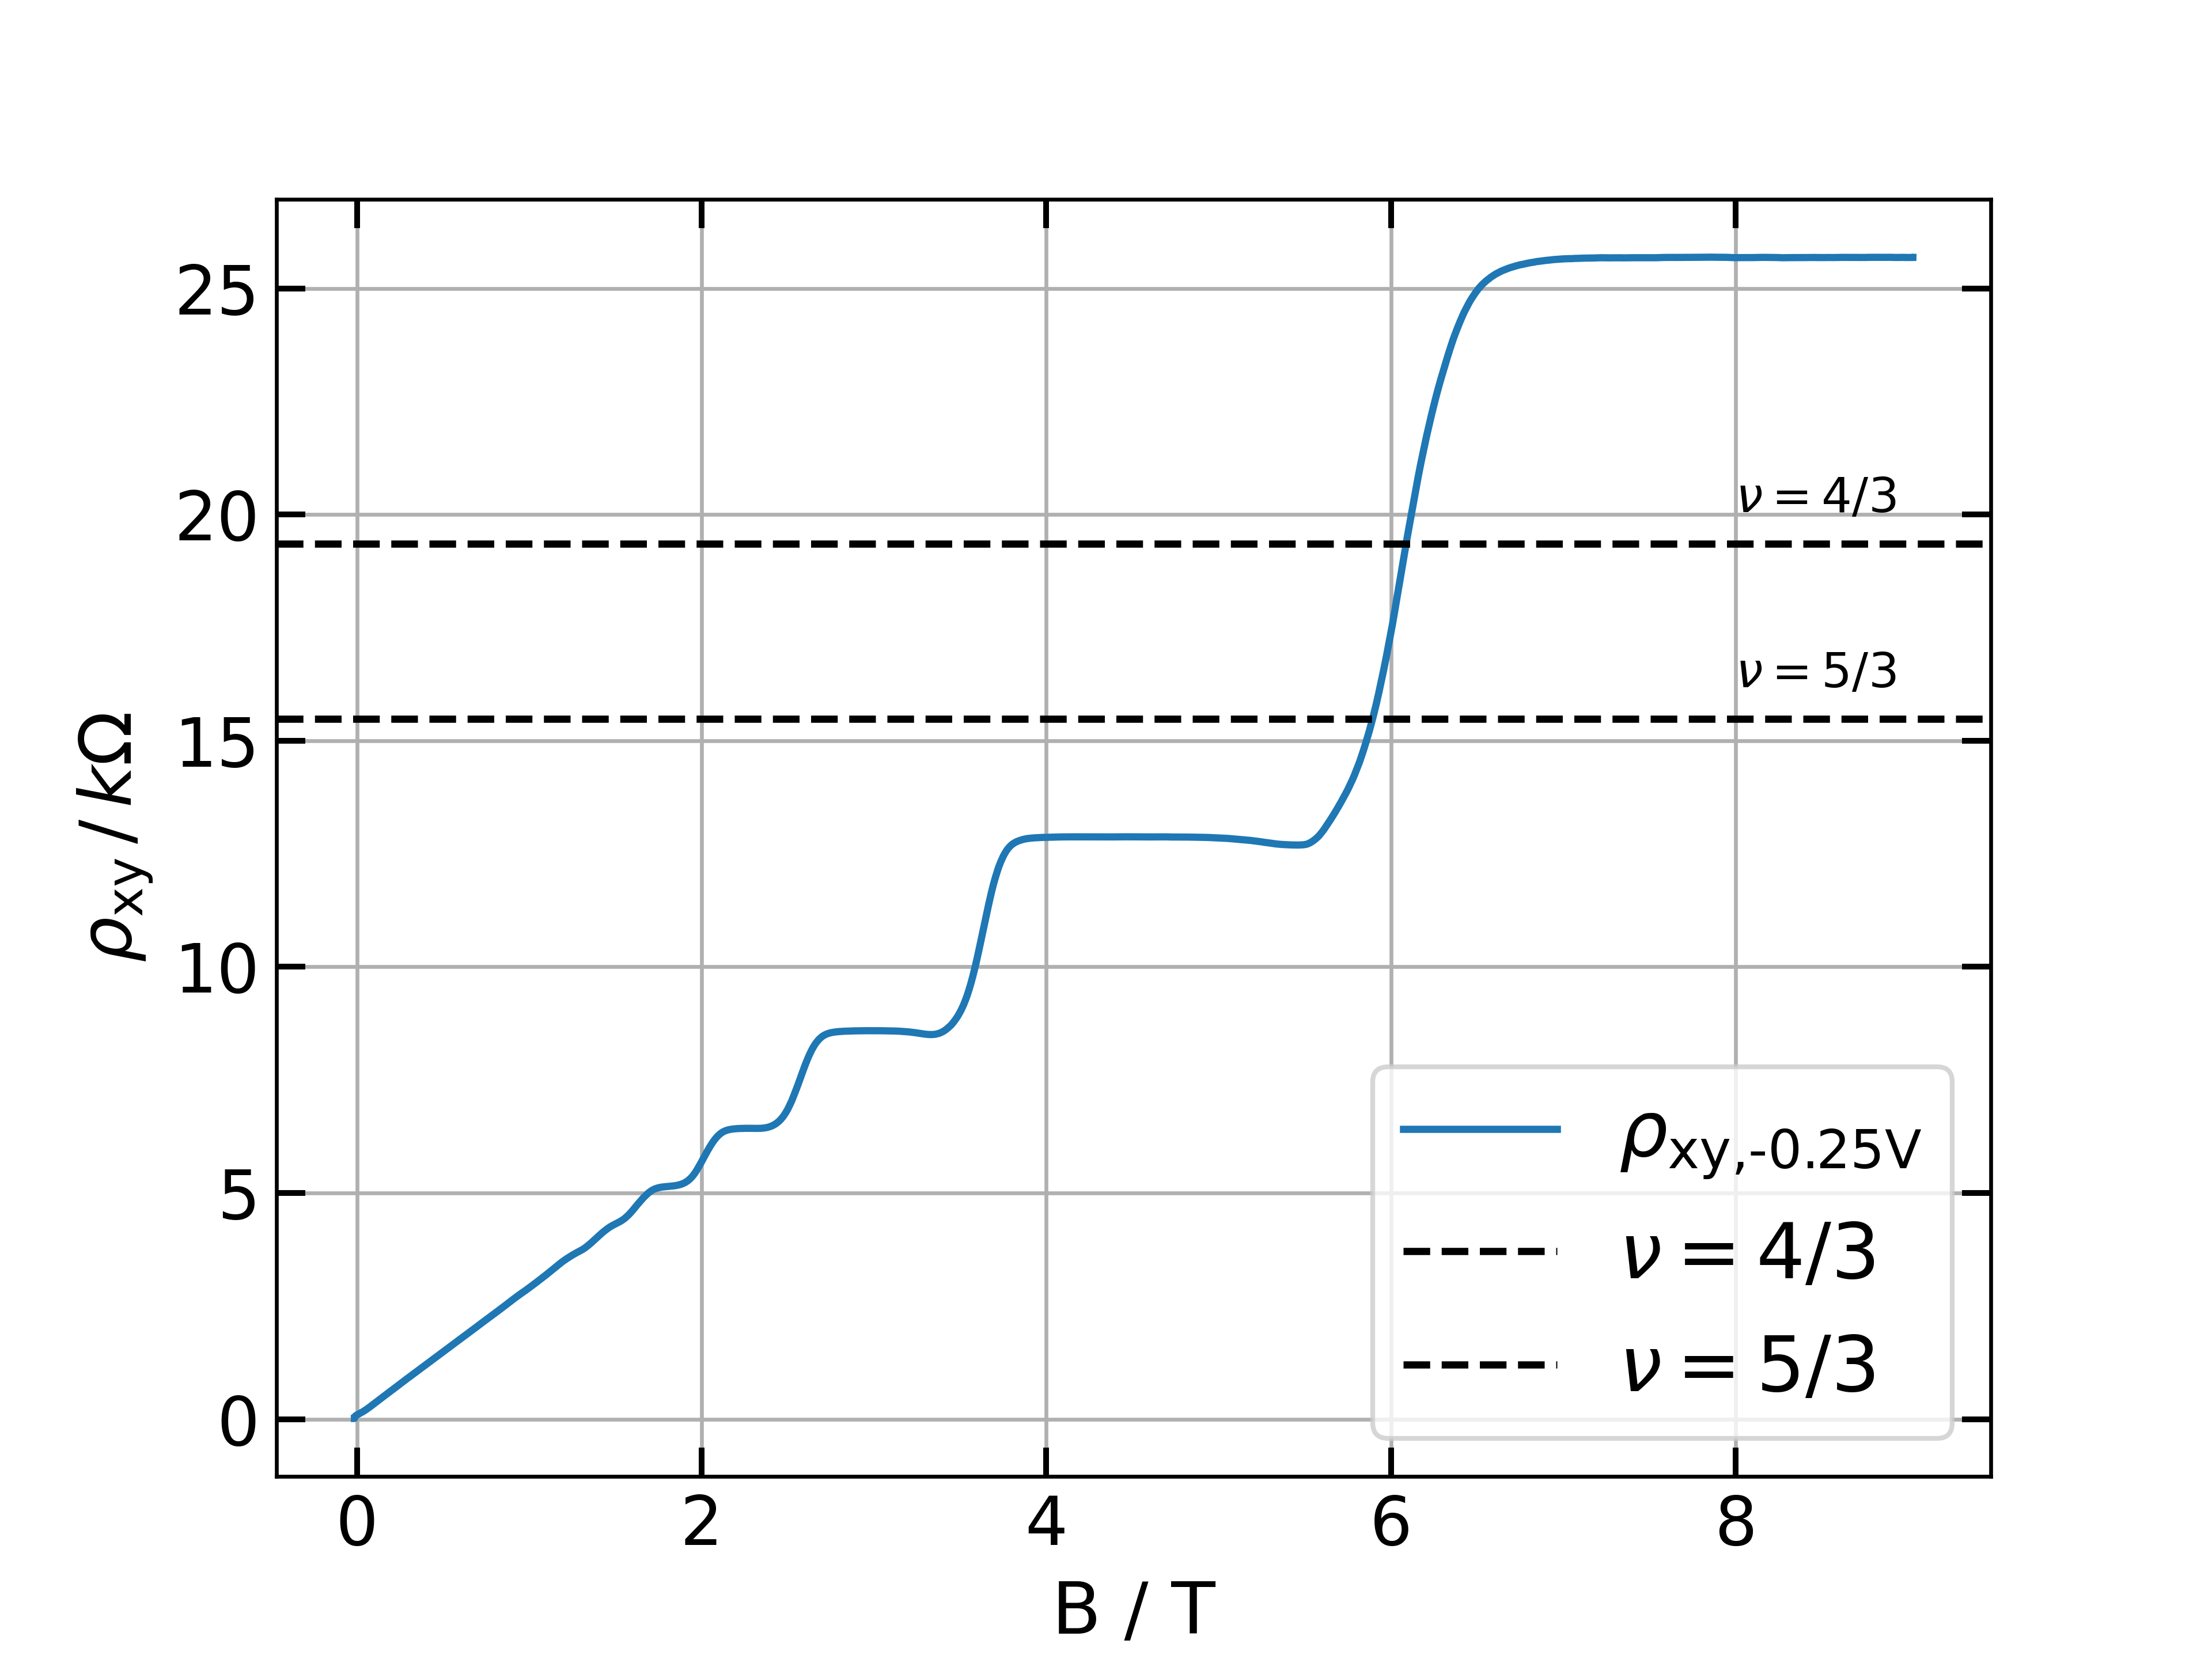
\includegraphics[width=0.45\textwidth]{../Images/FQHE.png}
    \caption{
        }
    \label{fig:FQHE}
\end{figure}
Also, the longitudinal resistivity shows no peaks between the large peaks corresponding to integer $\nu$.
In summary, there is no clear evidence for the fractional quantum Hall effect.







